\section{Theoretical Results} \label{sec:theory}  
We now describe the main technical results of this paper. 
In the first subsection we describe the setting under which the problem can be solved using the results which follow. 
\subsection{Topological Degree Theory}
Our results take advantage of the well studied area of topological degree theory. 
For an introduction to topological degree theory see the works of \cite{fonseca1995degree}, \cite{MoVrYa2002}, and \cite{OrChCh2006}.
It suffices to say that should $\Omega\subset\R^{n}$ be open and bounded, $F:\Omega\rightarrow \R$ continuous, differentiable, and $F(\vx) \neq \vy~\forall \vx\in\partial\Omega$ for some $\vy\in\R^n$, then the degree of $F$ at $\vy$ over $\Omega$, denoted $d\left(\Omega,F,\vy\right)\in\mathbb{Z}$, is defined. 
For the purposes of this article we utilize the following property of degree as our definition of the topological degree of a function $F$ at $\vy$ over a set $\Omega$. 
See O'Regan et al.~\cite{OrChCh2006} for details.
\begin{equation}\label{eq:Deg3}
  d\left(\Omega,F,\vy\right)=\sum\limits_{\vx\in F^{-1}(\vy)}\operatorname{sign}\left(J_F(\vx)\right)
\end{equation}
%
where $\operatorname{sign}\left(J_F(\vx)\right)$ denotes the sign of the Jacobian of $F$ at $\vx$, i.e.,
%
\[\operatorname{sign}\left(J_F(\vx)\right)=   \left\{
\begin{array}{ll}
       \ -1   & \mbox{if } J_F(\vx)< 0, \\
      \quad 0 & \mbox{if } J_F(\vx)= 0,~\mbox{ and } \\
      \quad 1 & \mbox{if } J_F(\vx)> 0. \\
\end{array} 
\right. \]
%
Additionally we utilize the following two common properties of the topological degree. 
Again, see O'Regan et al.~\cite{OrChCh2006} for details. 

If $H : [0,1]\times\bar{\Omega}\rightarrow\R^n$ is continuous such that $H(t,\vx)\neq \vy~\forall t\in[0,1],~\vx\in\partial\Omega$,  then 
\begin{equation}\label{eq:Deg1} 
  d\left(\Omega,H(t,\cdot),\vy\right)\text{ does not depend on }t.
\end{equation}

\begin{equation}\label{eq:Deg2}
  \text{If } d(\Omega,F,\vy) \neq 0, \text{ then there exists } \vx \in \Omega \text{ such that } F(\vx)=\vy. 
\end{equation}

\subsection{New Theoretical Results}
In this section we will take full advantage of properties (\ref{eq:Deg3}), (\ref{eq:Deg1}), and (\ref{eq:Deg2}) as they apply to the Robust Feasibility Problem.
We begin by assuming there is a unique solution to the forecasted system at which point the Jacobian is non-zero.
We conclude by property (\ref{eq:Deg3}) that the degree is non-zero at $\vu^*$ for the forecasted system. 
We then utilize property (\ref{eq:Deg1}) to equate the degree of $\vu$ to the degree of $\vu^*$ for all $\vu$ satisfying the limits specified in Equation (\ref{eq:uLimits}) (under a proposed robustness margin), which by property (\ref{eq:Deg2}) allows us to guarantee solutions to the system under all realizations of $\vu$ satisfying the limits (in \ref{eq:uLimits}), i.e., verify the system is robust feasible for a given robustness margin.
Invoking property (\ref{eq:Deg1}), however, requires us to develop a homotopy that captures the system under all possible realizations of $\vu$ satisfying the limits in (\ref{eq:uLimits}).
Once we define such a homotopy we reduce the Robust Feasibility Problem to the problem of verifying the hypothesis of property (\ref{eq:Deg1}). 

\medskip
To that end let $F(\vx)=Q(\vx)+L\vx$, $\Omega=\{\vx| A\vx \leq \vb\}$ and $\hat{\vx}\in \Int(\Omega)$ be a solution to the forecasted system $F(\vx)=\vu^*$ given in \cref{eq:Quad}, such that $\operatorname{sign}\left(J_{F}(\hat{\vx})\right) \neq 0$.
For a review of efficient methods of verification that could be used here, see the work of Griewank \cite{GRIEWANK2014}. 
If no solution exists, then certainly the system is not robust feasible.
We define $\Omega_u=\{\vu \,|\,\vu \text{ satisfies limits in \cref{eq:uLimits}}\}$.
Our task is then to verify using existing methods or those we propose in this paper that no other solutions exist in $\Int(\Omega)$.
This step may require further restricting the domain or even a slight perturbation of the forecasted $\vu$. 
Thus by property (\ref{eq:Deg3}) we have verified that $d\left(\Omega, F(\vx), \vu^*\right)\neq 0$. 
Note that this is not the only method for verification, but in some sense is the easiest to carry out for our purposes. 

\medskip
We now introduce the homotopy we use to invoke property (\ref{eq:Deg1}).
Let  $\ell_{\vu^*}$ represent an arbitrary line passing through $\vu^*$ and let $\vl_{\min}$ and $\vl_{\max}$ be the two points of intersection of $\partial\Omega_u$ and $\ell_{\vu^*}$.
We define a homotopy $H_{\ell_{\vu^*}} : [0,1]\times\bar{\Omega}\rightarrow\R^n$ as 
\begin{align}
  H_{\ell_{\vu^*}}(t,\vx) = F(\vx)-\left[(1-t)\vl_{\min}+t\vl_{\max}\right]\,. \label{eq:Homo}
\end{align}
Based on this homotopy, we present the key result on verification of robust solvability problem.
%in \cref{lem:NaScondition}.
%
%\add{
\begin{lem}
  \label{lem:NaScondition}
  Let $\Omega=\{\vx| A\vx \leq \vb \}$, $\Omega_u=\{\vu \,|\,\vu\, \text{satisfies limits in \cref{eq:uLimits}}\}$ and $F(\vx)=Q(\vx)+L\vx$,  as described in Equations (\ref{eq:Quad}), (\ref{eq:xLimits}), and (\ref{eq:uLimits}). 
  If $d(\Omega,H_\ell\left(\frac{1}{2},\vx\right), \vzero) \neq 0$ for each choice of $\ell = \ell_{\vu^*}$, then the system is robust solvable if and only if the following statement holds:
  \begin{align}
    \not\exists \vx\in\partial\Omega, \vu\in\Omega_u \ \ \mbox{ such that } \ F(\vx)-\vu=\vzero \,. \label{eq:RSForm}
  \end{align}
\end{lem}

\begin{proof}
%Let $\vl_{\min},\vl_{\max}$ be two points of intersection between $\partial\Omega_u$ and $\ell_{\vu^*}$. We define a homotopy $H_{\ell_{\vu^*}} : [0,1]\times\bar{\Omega}\rightarrow\R^n$ as 
%	\begin{align}
%		H_{\ell_{\vu^*}}(t,\vx) = F(\vx)-\left[(1-t)\vl_{\min}+t\vl_{\max}\right]\,. \label{eq:Homo}
%	\end{align}
  Since $d\left(\Omega, F(\vx), \vu^*\right)\neq 0$ is verified by property (\ref{eq:Deg3}), to show the problem is robust solvable, it follows by the fact that there exists a unique solution $\hat{\vx}\in \Int(\Omega)$ to the forecasted system given in \cref{eq:Quad} such that  $H_{\ell_{\vu^*}}\left(\frac{1}{2},\hat{\vx}\right)=F(\hat{\vx})-\vu^*=\vzero$ and $ \operatorname{sign}\left(J_{H_{\ell_{\vu^*},\frac{1}{2}}}(\hat{\vx})\right) \neq 0$.
  And this condition holds if and only if $d(\Omega,H_\ell\left(\frac{1}{2},\vx\right),\vzero)\neq 0$ according to property (\ref{eq:Deg2}).
  Note that this property holds for all such lines passing through $\vu^*$ since for each $\hat{\vu}\in\Omega_u\setminus\{\vu^*\}$, there exists a line $\hat{\ell}_{\vu^*}$ passing through $\vu^*$ and $t\in[0,1]$, such that $\hat{\vu}=(1-t)\hat{\vl}_{\min}+t\hat{\vl}_{\max}$.
  Thus, when $d(\Omega,H_\ell\left(\frac{1}{2},\vx\right),\vzero)\neq 0$ for each choice of $\ell_{\vu^*}$,   we have 
  \[
    d(\Omega,H_\ell\left(\frac{1}{2},\vx\right),\vzero)\neq 0 \, \Longleftrightarrow \,
    F(\vx) - \vu \neq \vzero, \forall \vx \in \partial\Omega, \vu \in \Omega_u \,.
  \]
  Hence the system is robust solvable if and only if the statement  (\ref{eq:RSForm}) holds.
\end{proof}
%}

Note that the statement (\ref{eq:RSForm}) is equivalent to property (\ref{eq:Deg1}) holding.
From here on we will assume $d(\Omega,H\left(\frac{1}{2},\vx\right),\vzero)\neq 0$ and focus our efforts on the development of methods for validating or invalidating the statement (\ref{eq:RSForm}).

\begin{lem} 
  \label{lem:BdOpt}
  Let $X\subset\R^n$ be compact. If $\vF:\R^n\rightarrow\R^n$ is continuous, and 
  \[
  \min\limits_{\norm{\vlambda}=1} \, \max\limits_{\vx\in X} \, \vlambda^T\vF(\vx)
  \]
  obtains its optimal value at $\hat{\vx}$ and $\vlambda_{\hat{\vx}}$ then $\vF(\hat{\vx})\in \partial \vF(X)$. 
\end{lem}

\begin{proof} 
  We get the result by arriving at a contradiction.
  Assume $\vF(\hat{\vx})\in \vF(X)\setminus\partial \vF(X)$. 
  Let $\theta$ the angle between $\vlambda_{\hat{\vx}}$ and $F(\hat{\vx})$. 
  Thus
  \[
  \min\limits_{\norm{\vlambda}=1}\max\limits_{\vx\in X}\ \vlambda^T\vF(\vx) ~=~ \vlambda_{\hat{\vx}}^T\vF(\hat{\vx}) ~=~ \norm{\vF(\hat{\vx})}\cos(\theta).
  \]
  Since $X\in\R^n$ is compact, $\vF(X)$ is also compact. 
  Hence there exists an $r>0$ such that  $B_r(\vF(\hat{\vx}))$, the ball of radius $r$ centered at $\vF(\hat{\vx})$, is in $\vF(X)\setminus\partial \vF(X)$. 
  Let $\vy$ be the antipodal point on $\partial B_r(\vF(\hat{\vx}))$ to the point of intersection between the line segment connecting the origin to $\vF(\hat{\vx})$ and $B_r(\vF(\hat{\vx}))$. 
  It follows then that $\norm{\vy}>\norm{\vF(\hat{\vx})}$ and $\theta$ is the angle between $\vlambda_{\hat{\vx}}$ and $\vy$.   
  Let $\vx^*\in X$ be such that $\vF(\vx^*)=\vy$.
  Such an $\vx^*$ exists since $\vF(X)$ is compact. 
  Therefore $\vlambda_{\hat{\vx}}^T\vF(\vx^*)=\norm{\vF(\vx^*)} \cos(\theta) > \norm{\vF(\hat{\vx})} \cos(\theta) = \vlambda_{\hat{\vx}}^T\vF(\hat{\vx})$, which is a contradiction. 
  The lemma now follows.
\end{proof}

%\add{
We illustrate \cref{lem:BdOpt} in \cref{fig:illustration}.
The compact set $X\subset\R^2$ is shown in pink with boundary shown in blue.
For continuous $\vF:\R^2 \rightarrow \R^2$, let $\hat{\vx}$ be the point and $\vlambda_{\hat{\vx}}$ the unit vector that give the optimal value of $\min_{\norm{\vlambda}=1} \, \max_{\vx\in X} \, \vlambda^T\vF(\vx)$ as $\vlambda_{\hat{\vx}}^T\vF(\hat{\vx})$ based on \cref{lem:BdOpt}.
These vectors are shown in red.
In the case when the origin is contained in $\vF(\vx)$, as it happens here, we observe that there exists another point $\vx$ and unit vector $\vlambda_{\vx}$ satisfying $\vF(\vx) \in \partial \vF(X)$ (and thus $\vx\in \partial X$) such that we can get the lower bound of $\min_{\norm{\vlambda}=1}\max_{\vx\in X}\ \vlambda^T\vF(\vx)$ as $\min_{\vx\in \partial X} \max_{\norm{\vlambda}=1}\ \vlambda^T\vF(\vx)$ (shown in green).
%}

\begin{figure}[htp!]
\begin{center}
  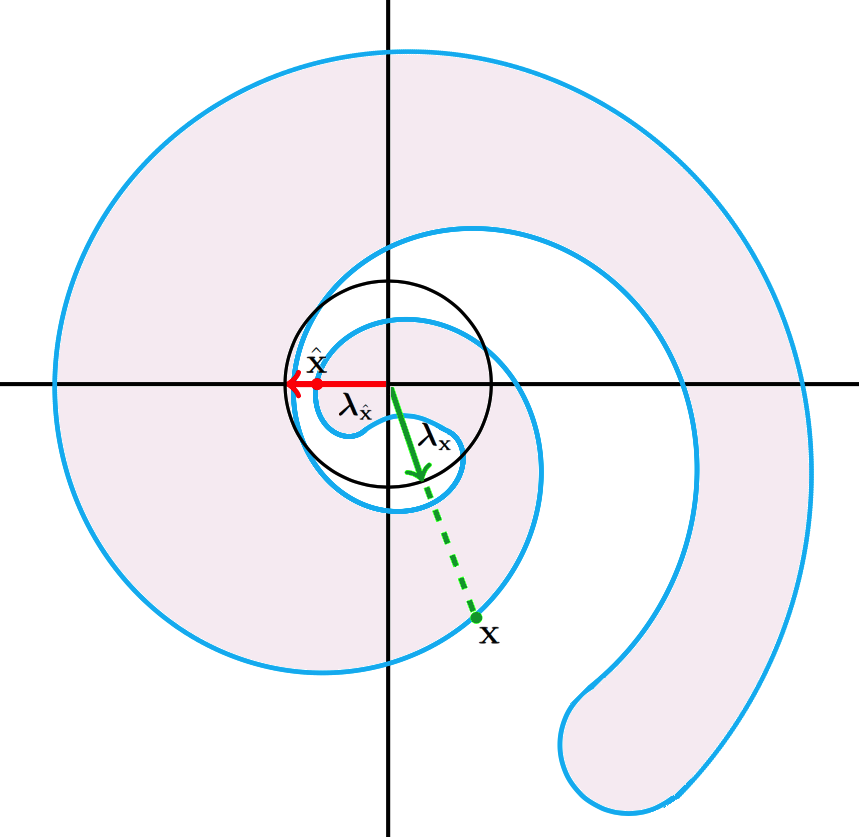
\includegraphics[scale=0.32]{illustration.png}
\end{center}
\caption{\label{fig:illustration}
  Illustration of \cref{lem:BdOpt}.
  The unit vectors $\vlambda_{\hat{\vx}}$ and $\vlambda_{\vx}$ are shown as the red and green arrows, respectively.
}
\end{figure}

We formalize the last observation for the general case in our main theorem, which characterizes the structure of the function $\vF$.

\begin{thm} 
  \label{thm:MainIneq}
  Let $X\subset\R^n$ be compact, $\vF:\R^n\rightarrow\R^n$ be continuous such that $\vF(X)$ contains the origin. 
  If $\vF$ is injective over $X$ then
  \[
  \min\limits_{\norm{\vlambda}=1}\max\limits_{\vx\in X}\ \vlambda^T\vF(\vx) ~\geq~ \min\limits_{\vx\in \partial X} \max\limits_{\norm{\vlambda}=1}\ \vlambda^T\vF(\vx).
  \]
  %
  %\smallskip
  \begin{proof}
    Consider the origin lies on the boundary of $\vF(X)$, and let $\hat{\vx} \in \partial X$ such that $F(\hat{\vx})=\vzero$. 
    Such an $\hat{\vx}$ exists since $\partial F(X) = F(\partial X)$ by the Invariance of Domain theorem, as $F$ is continuous and injective over a compact set (so, an interior point cannot get mapped to a boundary point). 
    Then  clearly
    \[
       \min\limits_{\norm{\vlambda}=1}\max\limits_{\vx\in X}\ \vlambda^T\vF(\vx) ~\geq~
       \min\limits_{\norm{\vlambda}=1}\vlambda^T\vF(\hat{\vx}) ~=~ 0 ~=~
       \max\limits_{\norm{\vlambda}=1}\ \vlambda^T\vF(\hat{\vx}) ~\geq~
       \min\limits_{\vx\in \partial X}\max\limits_{\norm{\vlambda}=1}\ \vlambda^T\vF(\vx).
    \]
    Hence assume the origin lies in the interior of $\vF(X)$.
    Let $\hat{\vx}$ be the point and $\vlambda_{\hat{\vx}}$ the unit vector at which
    \[
    \min\limits_{\norm{\vlambda}=1}\max\limits_{\vx\in X}\ \vlambda^T\vF(\vx)
    \]
    obtains its optimal value.
    We consider two cases.

    Case 1: If the angle $\theta$ between $F(\hat{\vx})$ and $\vlambda_{\hat{\vx}}$ is $0$, then $\displaystyle \max\limits_{\norm{\vlambda}=1}\vlambda^T\vF(\hat{\vx}) = \vlambda_{\hat{\vx}}^T\vF(\hat{\vx})$. 
    Furthermore by \cref{lem:BdOpt}, $\vF(\hat{\vx}) \in \partial \vF(X)$ and thus $\hat{\vx}\in \partial X$ since $\vF$ is injective, i.e., $\vF$ maps $\partial X$ to $\partial \vF(X)$, by hypothesis. 
    It follows now that
    \[
      \min\limits_{\vx\in \partial X}\max\limits_{\norm{\vlambda}=1}\ \vlambda^T\vF(\vx) ~\leq~
      \max\limits_{\norm{\vlambda}=1}\ \vlambda^T\vF(\hat{\vx}) ~=~
      \vlambda_{\hat{\vx}}^T\vF(\hat{\vx}) ~=~
      \min\limits_{\norm{\vlambda}=1}\max\limits_{\vx\in X}\ \vlambda^T\vF(\vx).
    \]

    Case 2: Assume the angle $\theta \neq 0$ (between $F(\hat{\vx})$ and $\vlambda_{\hat{\vx}}$). 
    Let $\vx^*$ be a point on the boundary of $X$ such that the angle between $\vlambda_{\hat{\vx}}$ and $\vF(\vx^*)$ is 0. 
    Such a point must exist as $\vF(X)$ is compact and by hypothesis $\vF(X)$ contains the origin, is injective,
    %i.e., $\vF$ maps $\partial X$ to $\partial \vF(X)$,
    and by assumption the origin lies in the interior of $\vF(X)$. 
    It follows then that
    \[
      \min\limits_{\vx\in \partial X}\max\limits_{\norm{\vlambda}=1}\ \vlambda^T\vF(\vx) ~\leq~
      \max\limits_{\norm{\vlambda}=1}\vlambda^T \vF(\vx^*) ~=
      \vlambda_{\hat{\vx}}^T\vF(\vx^*) ~\leq
      \max\limits_{\vx\in X}\vlambda_{\hat{\vx}}^T\vF(\vx) ~=~
      \min\limits_{\norm{\vlambda}=1}\max\limits_{\vx\in X}\ \vlambda^T\vF(\vx).
    \]
    The theorem now follows.
  \end{proof}
\end{thm}

\cref{thm:MainIneq} and \cref{lem:BdOpt} provide us with the theoretical tools we need to develop procedures for approximating the robustness margin.
The hypothesis of \cref{thm:MainIneq} does however require us to assume the system is injective under the constraints in Equation (\ref{eq:xLimits}).
However, injectivity is only required to ensure $\partial F(X) = F(\partial X)$, and thus we can generalize to systems that are not necessarily injective if they yet retain $\partial F(X) = F(\partial X)$ as an applicable property. 
With this in mind we carry with us the necessary property $\partial F(X) = F(\partial X)$ throughout the rest of the article. 
%There is room to improve here especially if there is a unique solution at u^* as this will still gaurantee the validity of the lower bd, but not necessarily that of the upper bd

We will use the terminology \enquote{inner bound procedures} to describe the processes of verifying robust feasibility while expanding the uncertainty box centered at $\vu^*$ in order to compute the lower bounds on the robustness margin, which these procedures undertake. 
We use the terminology \enquote{outer bound procedures} to capture in a similar fashion the procedures used to compute the upper bounds on the robustness margin by contracting the uncertainty box until the system may be robust feasible. 
As such we dedicate the next two sections to the development of these inner and outer bound formulations. 
